\subsubsection{Percentage of Time Spent on Top 10 Most Visited }

%===========================================================================
% Tabulated splits by party and by percentiles for hours spent on adultsites
%===========================================================================
\begin{table}[ht] \centering \small \setlength\tabcolsep{10 pt}
	\caption{Distribution of Consumption of Pornography Online by Party (\texttt{piedomains})}
	\label{tab:piedomains_distribution_duration_party}
	\begin{adjustbox}{max width=\textwidth}
		\begin{tabular}{crr}
			\toprule
			\multicolumn{1}{l}{\textbf{}}&\multicolumn{2}{c}{\textbf{Hours}}\\
			\cmidrule(l){2-3}
			\multicolumn{1}{l}{\textbf{Percentile}}&\multicolumn{1}{c}{\textbf{Republicans}}&\multicolumn{1}{c}{\textbf{Democrats}}\\
			\midrule
			0.00 &  0.0 &  0.0 \\
0.10 &  0.0 &  0.0 \\
0.20 &  0.0 &  0.0 \\
0.30 &  0.1 &  0.0 \\
0.40 &  0.2 &  0.1 \\
0.50 &  0.6 &  0.2 \\
0.60 &  1.1 &  0.4 \\
0.70 &  1.8 &  0.9 \\
0.80 &  3.4 &  2.0 \\
0.90 &  6.4 &  5.0 \\
0.95 & 16.3 &  7.8 \\
0.96 & 18.7 &  9.9 \\
0.97 & 24.0 & 13.1 \\
0.98 & 29.9 & 18.4 \\
0.99 & 31.7 & 33.4 \\
1.00 & 33.7 & 34.4 \\
			\bottomrule
		\end{tabular}
	\end{adjustbox}
	\caption*{\footnotesize \emph{Notes:} 
		The table shows splits by party and by key percentiles (each of the ten deciles plus quantiles at the right tail) for the duration (hours) spent by individuals who consumed pornography in the sample period. 
		Classification of pornography sites is based on a machine learning classifier \citep{Chintalapati_piedomains_Predict_the_2022}.
		See \cref{tab:piedomains_distribution_prop_duration_party} for the corresponding distribution in terms of percentage of time. 
		A two-sample Kolmogorov–Smirnov test returns a p-value of 0.0481, rejecting the null that the Republican and Democrat distributions are the same at the 5\% level.
		%See \cref{fig:distribution_duration_party} for the plot.
	}
\end{table}

%===============================================================================
% Tabulated splits by party and by percentiles for proportion of time spent on adultsites
%===============================================================================
\begin{table}[ht] \centering \small \setlength\tabcolsep{10 pt}
	\caption{Percentage of Time Spent on Pornographic Sites by Party (\texttt{piedomains})}
	\label{tab:piedomains_distribution_prop_duration_party}
	\begin{adjustbox}{max width=\textwidth}
		\begin{tabular}{crr}
			\toprule
			\multicolumn{1}{l}{\textbf{}}&\multicolumn{2}{c}{\textbf{\% time}}\\
			\cmidrule(l){2-3}
			\multicolumn{1}{l}{\textbf{Percentile}}&\multicolumn{1}{c}{\textbf{Republicans}}&\multicolumn{1}{c}{\textbf{Democrats}}\\
			\midrule
			0.00 &  0.0 &  0.0 \\
0.10 &  0.0 &  0.0 \\
0.20 &  0.1 &  0.0 \\
0.30 &  0.2 &  0.1 \\
0.40 &  0.5 &  0.3 \\
0.50 &  1.1 &  0.7 \\
0.60 &  3.4 &  1.4 \\
0.70 &  5.4 &  3.0 \\
0.80 & 10.8 &  7.1 \\
0.90 & 33.4 & 18.2 \\
0.95 & 42.1 & 41.9 \\
			\bottomrule
		\end{tabular}
	\end{adjustbox}
	\caption*{\footnotesize \emph{Notes:} 
		The table shows splits by party and by key percentiles (each of the ten deciles plus quantiles at the right tail) for the percentage of time spent on pornography by individuals who consumed pornography in the sample period. 
		Classification of pornography sites is based on a machine learning classifier \citep{Chintalapati_piedomains_Predict_the_2022}.
		See \cref{tab:piedomains_distribution_duration_party} for the corresponding distribution in terms of percentage of time.
		A two-sample Kolmogorov–Smirnov test returns a p-value of 0.19, failing to reject the null that the Republican and Democrat distributions are the same at the 5\% level.
		%See \cref{fig:distribution_prop_duration_party} for the plot.
	}
\end{table}

%====================================
% Figure of traffic to top x websites
%====================================
\begin{figure}[h]
	\centering
	\caption{Traffic to Top x Pornographic Sites by Party}
	\includegraphics[width=.6\textwidth]{figs/concentration_porn_consumption_topX_by_party.pdf}
	\caption*{\footnotesize \emph{Notes:} 
		The figure shows the concentration of pornography consumption based on individuals' most frequented pornographic sites.
            The underlying data is the individual's own most frequented site.
            We first sort online pornography sites for each individual and compute the percentage of time that individual spent for his/her own top 10 sites before computing and plotting the average (as shown above).
		Shaded areas are 95\% confidence intervals from bootstrapped standard errors (n = 1,000).
	}
	\label{fig:concentration_porn_consumption_topX_by_party}
\end{figure}

\begin{figure}[ht]
\caption{Time Spent on Online Pure Pornography vs. Adult-related Leisure}
\label{fig:tu_prop_adult_entertainment-prop_pure_adult}
     \centering
     \begin{subfigure}[b]{0.495\textwidth}
         \centering
         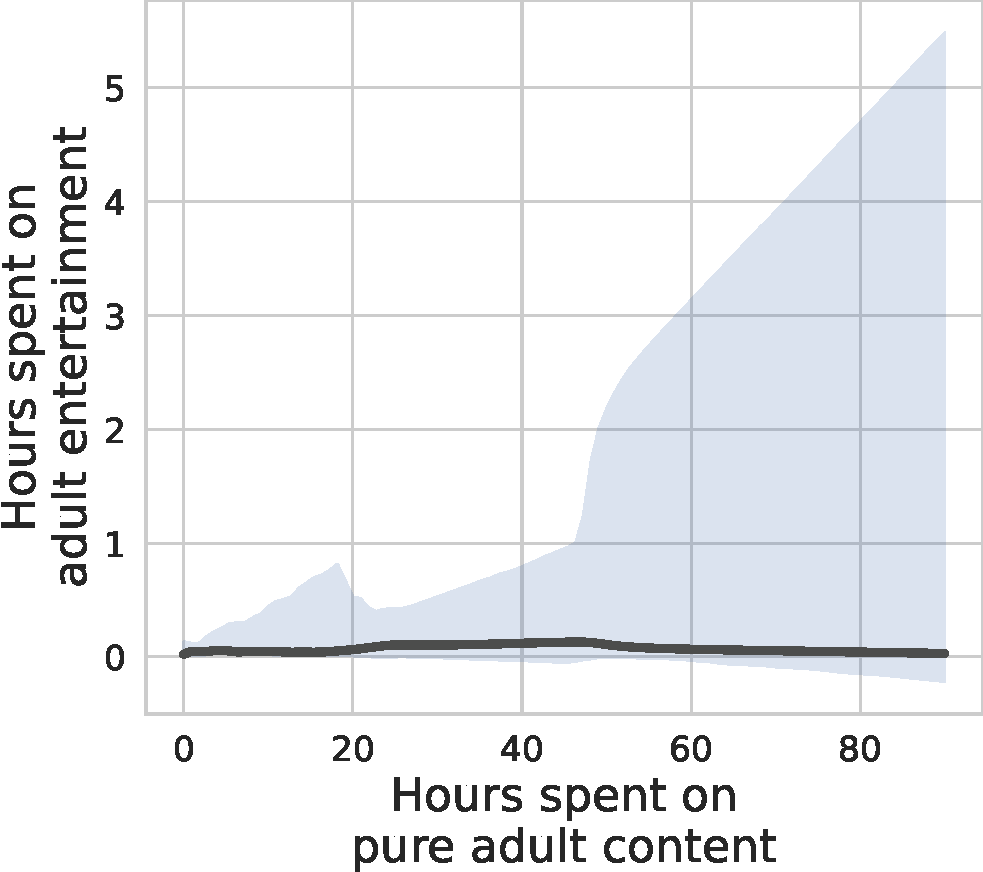
\includegraphics[width=\textwidth]{figs/tu_duration_adult_entertainment-duration_pure_adult.pdf}
         \caption{Entertainment}
     \end{subfigure}
     \hfill
     \begin{subfigure}[b]{0.495\textwidth}
         \centering
         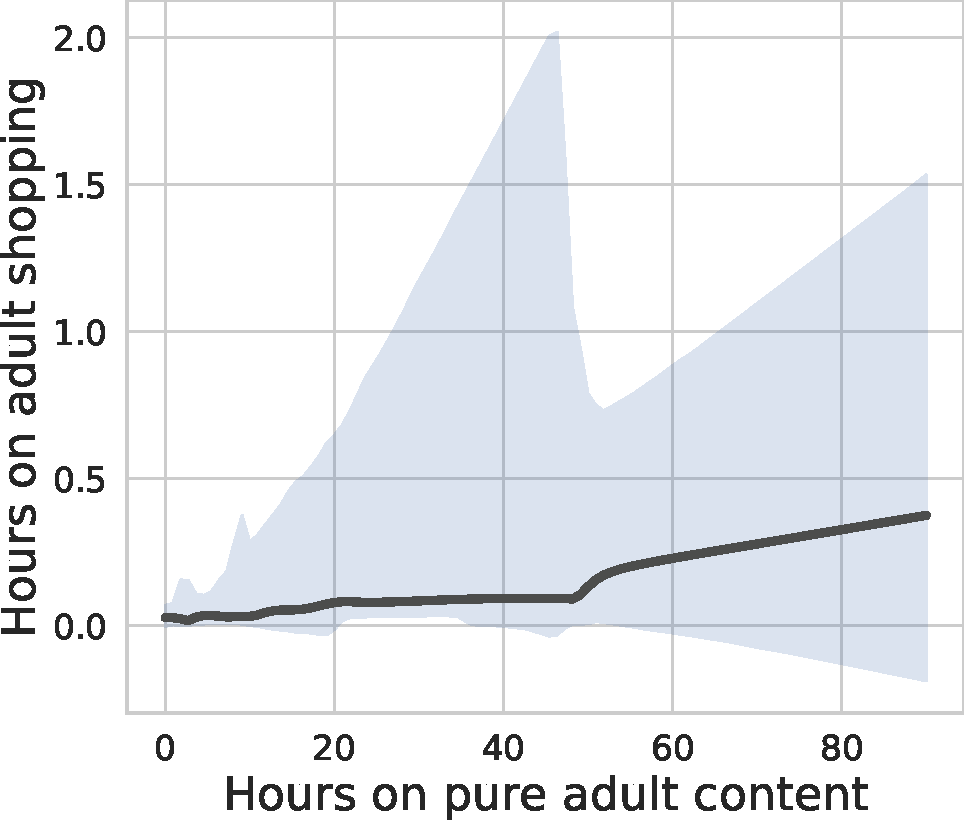
\includegraphics[width=\textwidth]{figs/tu_duration_adult_shop-duration_pure_adult.pdf}
         \caption{Shopping}
     \end{subfigure}
\caption*{\footnotesize \emph{Notes:}
Lowess for time spent on online pornography (excludes adult entertainment, adult gaming, adult shopping) vs time spent on other adult-related leisure (``adult entertainment'' and ``adult shopping'').
Observations above the 90th percentile are omitted. 
Adult-related entertainment sites are those with YouGov categories containing ``adult'' and ``entertainment''---top five of such sites are thechive.com, redgifs.com, 4chan.org, hentairead.com, and hentaifox.com. Adult-related shopping sites are those with YouGov categories containing ``adult'' and ``shopping''---top five of such sites are manyvids.com, adameve.com, victoriassecret.com, honeyplaybox.com, and r18.com. Each estimation in the Lowess uses half of the sample data. The 95\% confidence intervals shaded in blue are bootstrapped (n = 1000).}
\end{figure}


%% given sample size, probably misleading so I propose scraping it for now


%============================================================================
% Map of porn consumption (visits and duration)
%============================================================================
\begin{figure}[t]
	\caption{Porn Consumption by State}
	\label{fig:map_porn}
	\centering
	\begin{subfigure}[t]{0.8\textwidth}
		\centering
		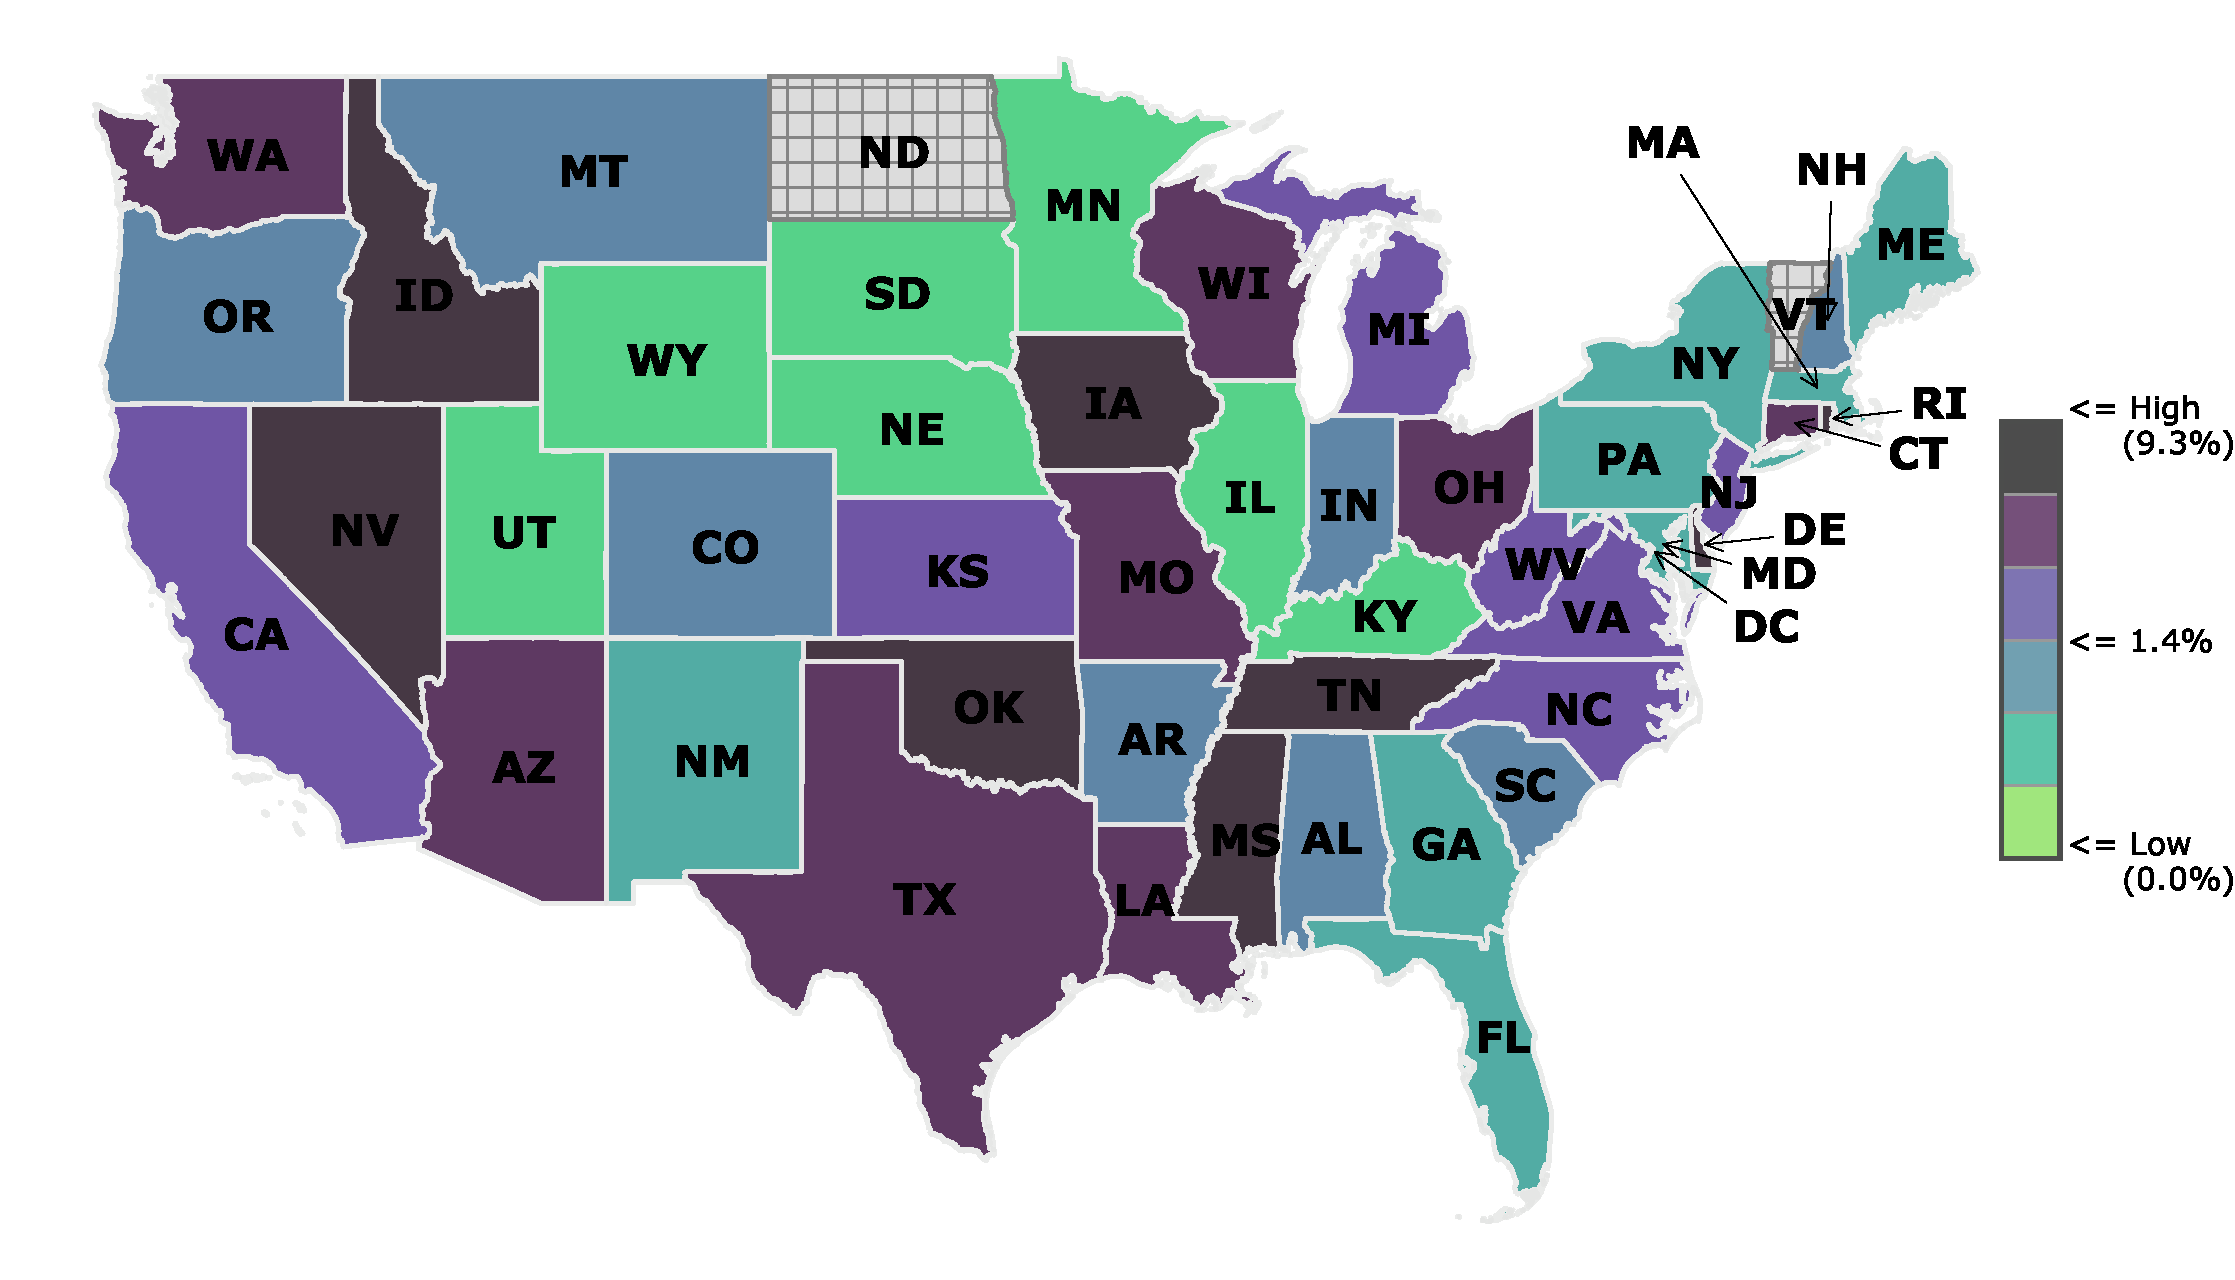
\includegraphics[width=\textwidth]{../figs/map_visits.pdf}
		\caption{Percentage of visits to porn sites}
	\end{subfigure}
	\begin{subfigure}[t]{0.8\textwidth}
		\centering
		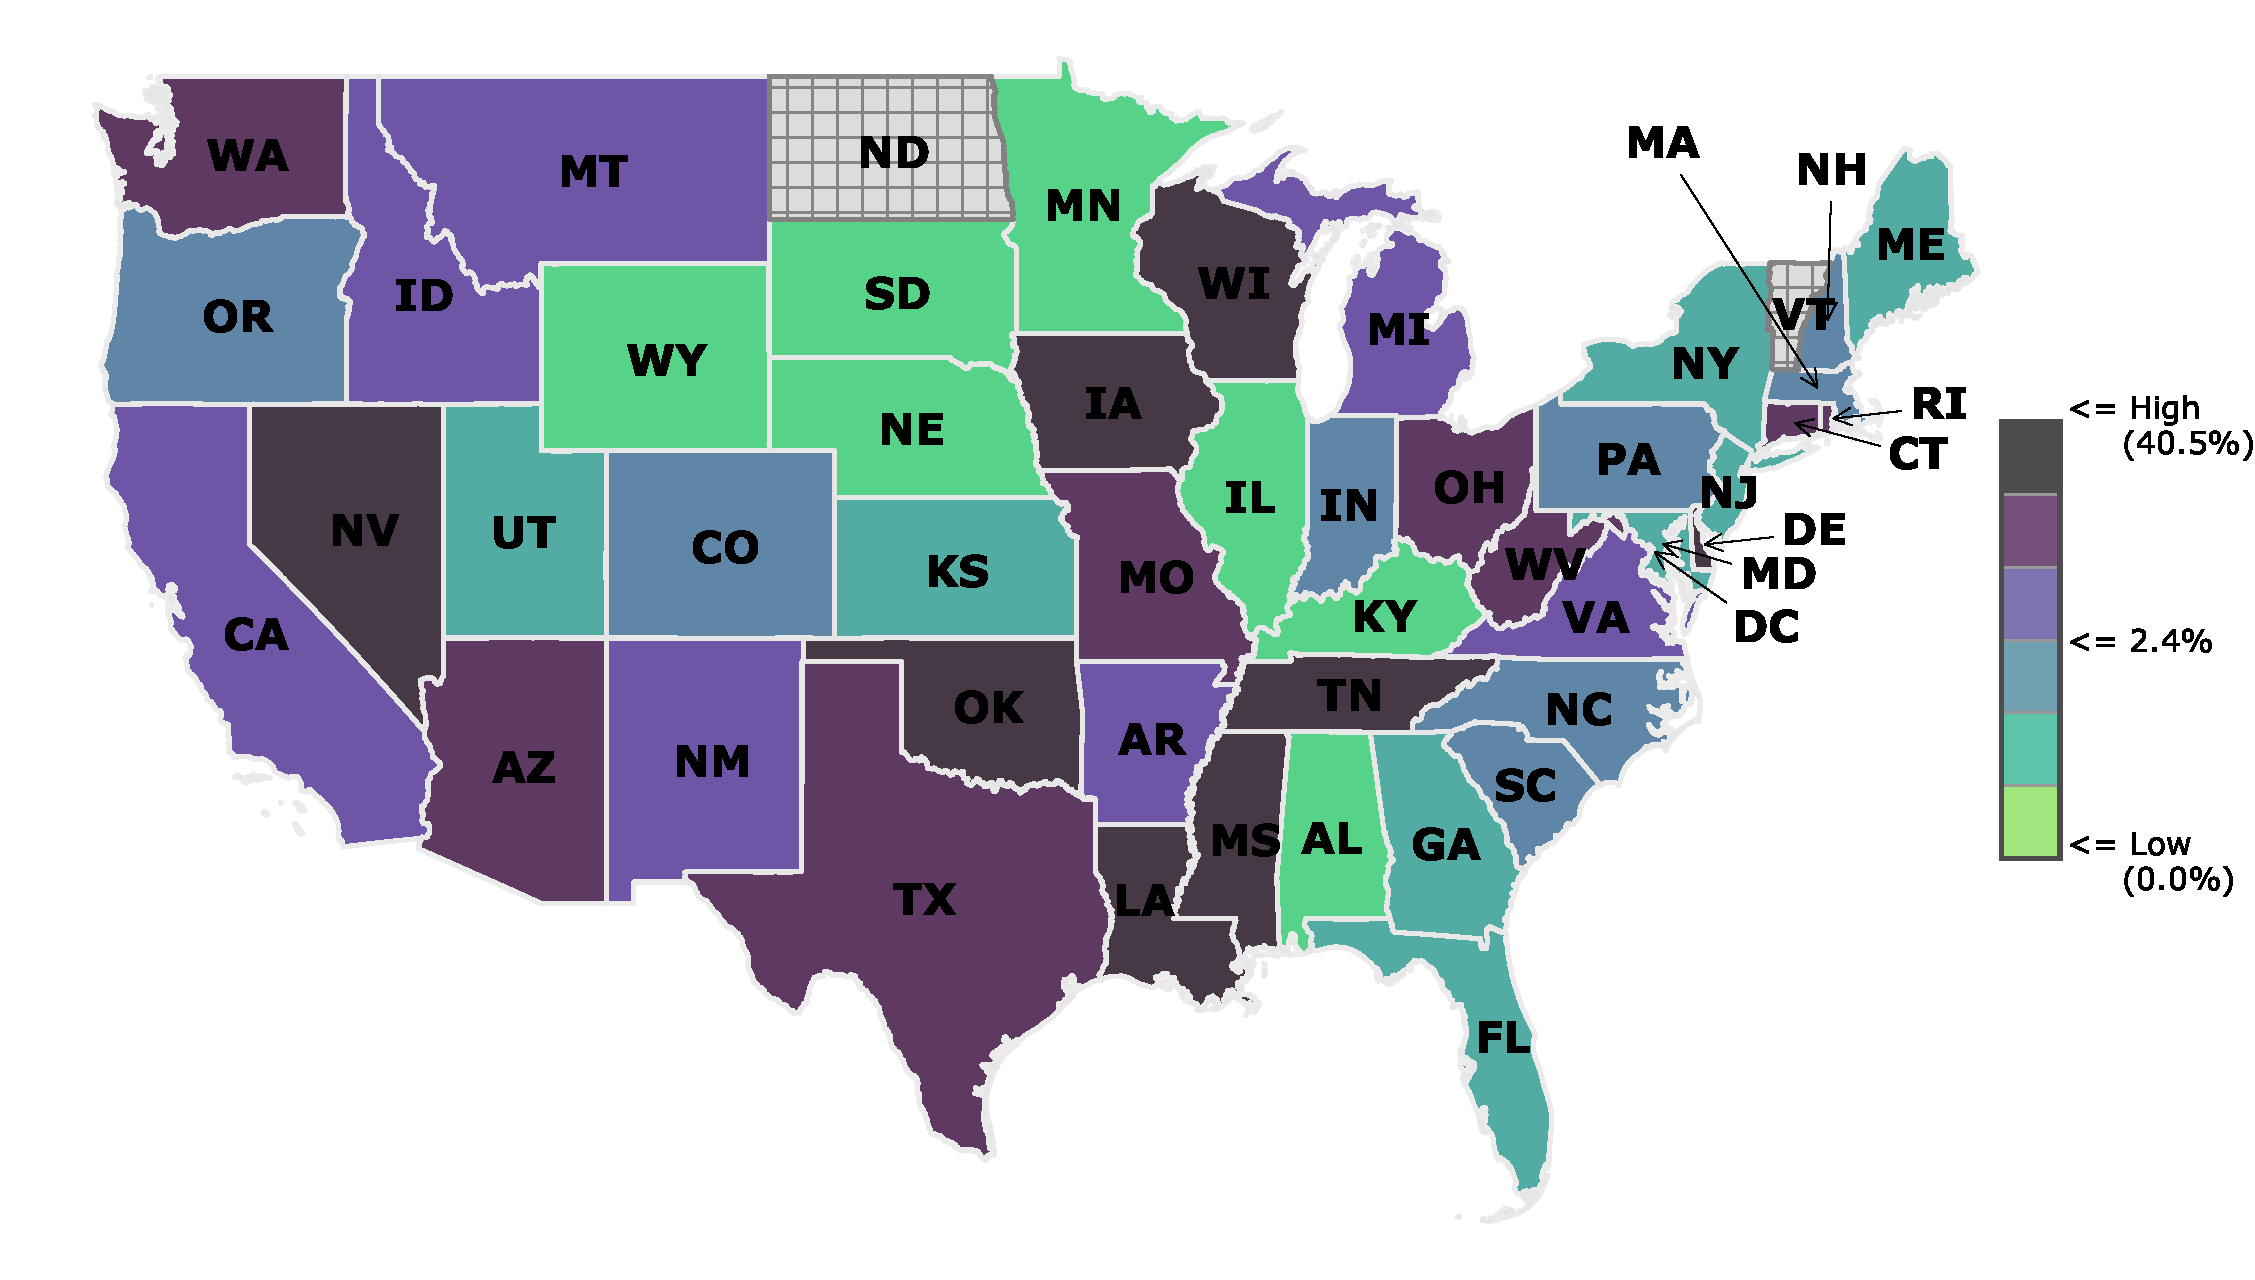
\includegraphics[width=\textwidth]{../figs/map_duration.pdf}
		\caption{Percentage of duration on porn sites}
	\end{subfigure}
	\caption*{\footnotesize \emph{Notes:} 
		Darker shades indicate higher values.
		Values for each state are percentage of visits to and time spent on porn sites averaged across individuals of the states.
		Baseline values are for all web browsing activity.
		North Dakota and Vermont have no data (shaded out).}
\end{figure}

\FloatBarrier

%% i didn't get the point of this so removing it for now

%======================================================
% Figure for concentration of porn consumption by party
%======================================================
\begin{figure}
	\centering
	\caption{Traffic to Top 10 Porn Sites by Party}
	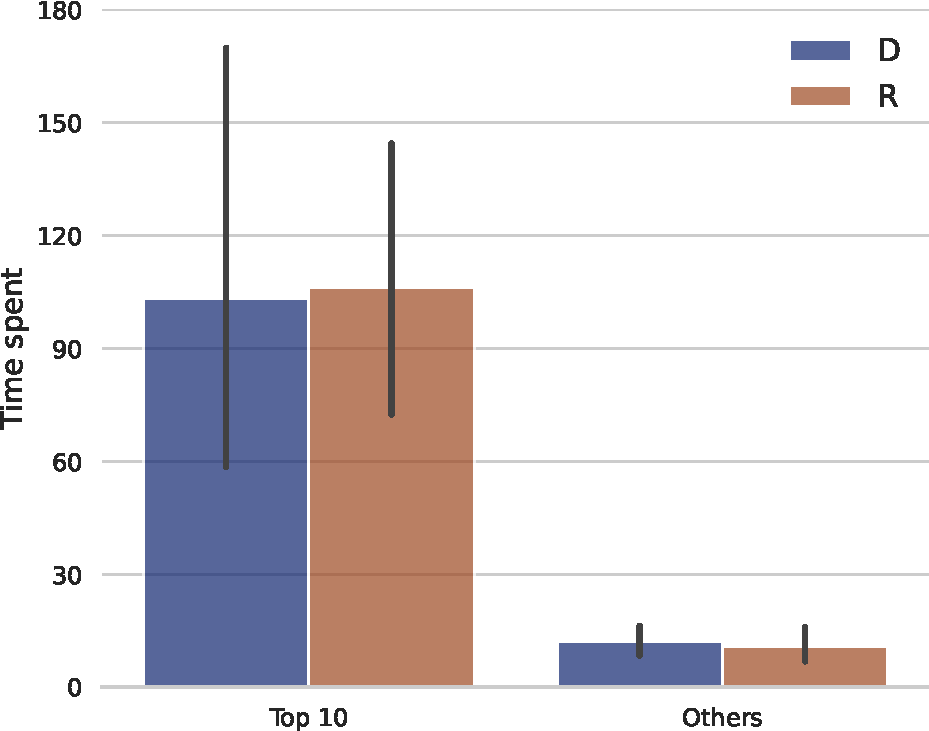
\includegraphics[width=.6\textwidth]{../figs/concentration_porn_consumption_by_party.pdf}
	\caption*{\footnotesize \emph{Notes:} 
		The Top 10 bar indicates traffic to the top 10 porn sites in the data (see \cref{fig:top25_adult}).
		The Others bar indicates traffic to all other porn sites outside of the top 10.
		The y-axis is the total time spent on porn sites, averaged across individuals.
		Time units is hours.
		Vertical bars are 95\% confidence intervals from bootstrapped standard errors (n = 1,000).
	}
	\label{fig:concentration_porn_consumption_by_party}
\end{figure}

%======================================================
% Figure for Distribution of Hours spent on adult sites
%======================================================
\begin{figure}[ht]
\centering
\caption{Distribution of Consumption of Pornography Online}
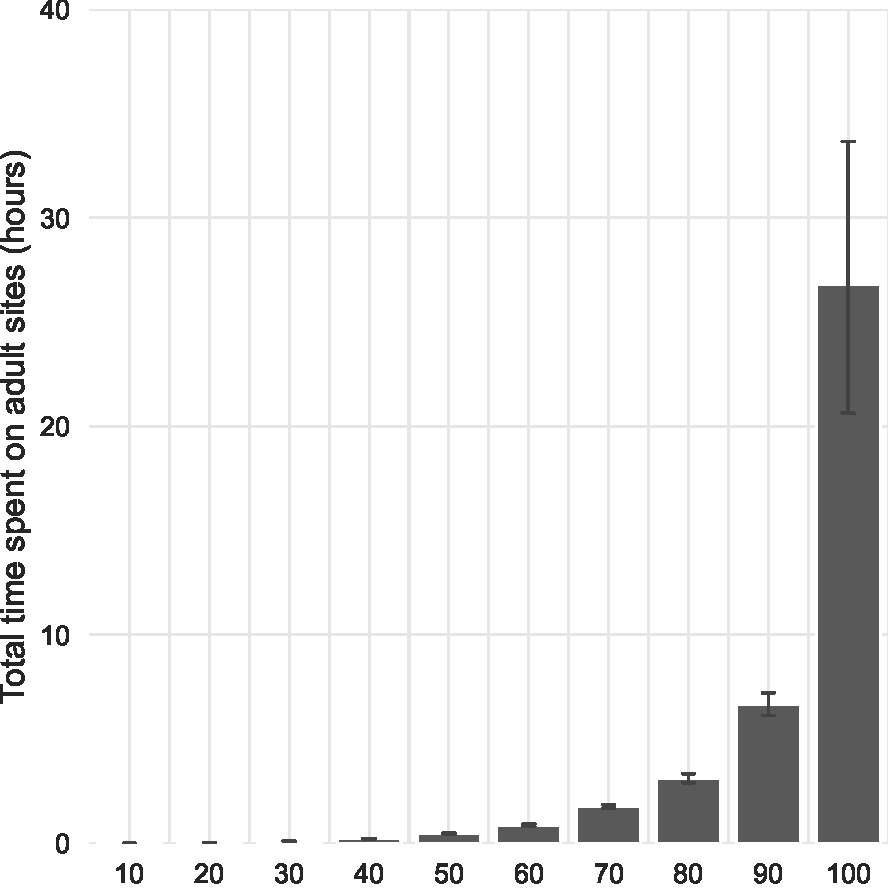
\includegraphics[width=.5\linewidth]{../figs/distribution_duration_on_adultsites.pdf}
\caption*{\footnotesize \emph{Notes:} 
	Figure shows the number of hours spent on pornographic sites by individuals who consumed pornography in the sample period.
	Individuals are split into deciles with each bin containing approximately the same number of individuals.
	Height of bars indicate mean of each bin.
	Capped vertical bars are 95\% confidence intervals.
	See \cref{tab:distribution_duration} for the more tabulated values.
}
\label{fig:distribution_duration}
\end{figure}

%===================================================================
% Figure for Distribution of proportion of time spent on adult sites
%===================================================================
\begin{figure}[ht]
	\centering
	\caption{Percentage of Time Spent on Pornographic Sites}
	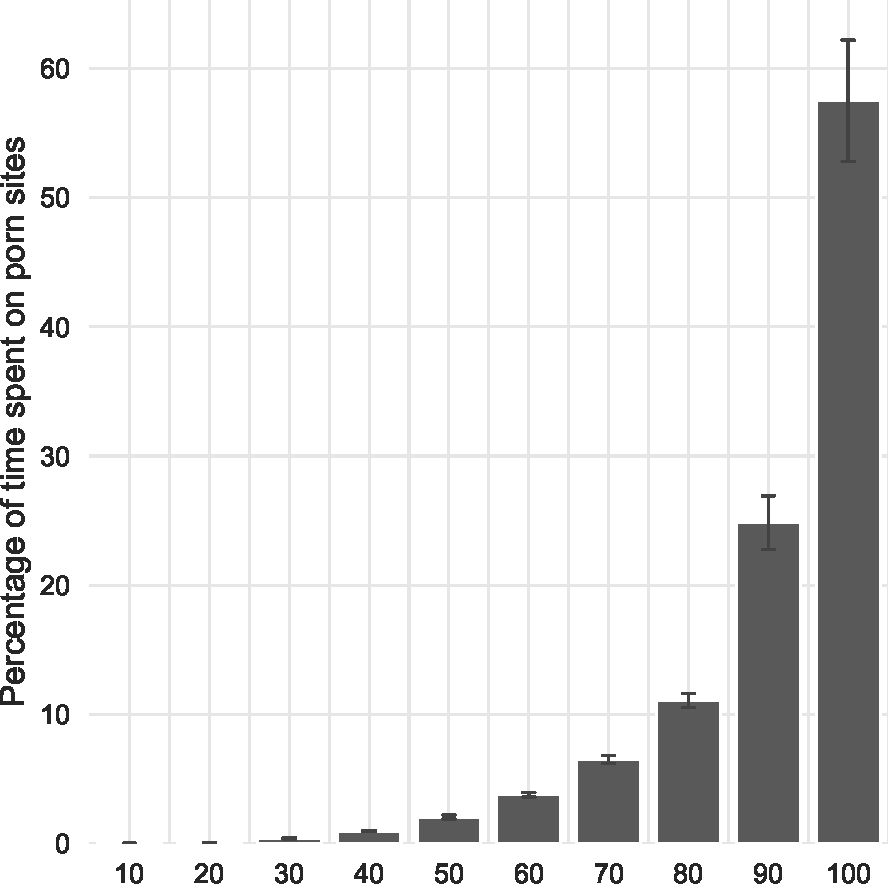
\includegraphics[width=.5\linewidth]{../figs/distribution_proportion_duration_on_adultsites.pdf}
	\caption*{\footnotesize \emph{Notes:} 
		Figure shows the proportion of time spent on pornographic sites by individuals who consumed pornography in the sample period.
		Individuals are split into deciles with each bin containing approximately the same number of individuals.
		Height of bars indicate mean of each bin.
		Capped vertical bars are 95\% confidence intervals.
		See \cref{tab:distribution_prop_duration} for the more tabulated values.
	}
	\label{fig:distribution_prop_duration}
\end{figure}

%===============================================
% Splits by party for hours spent on adult sites
%===============================================
\begin{figure}[ht]
	\centering
	\caption{Distribution of Consumption of Pornography Online by Party}
	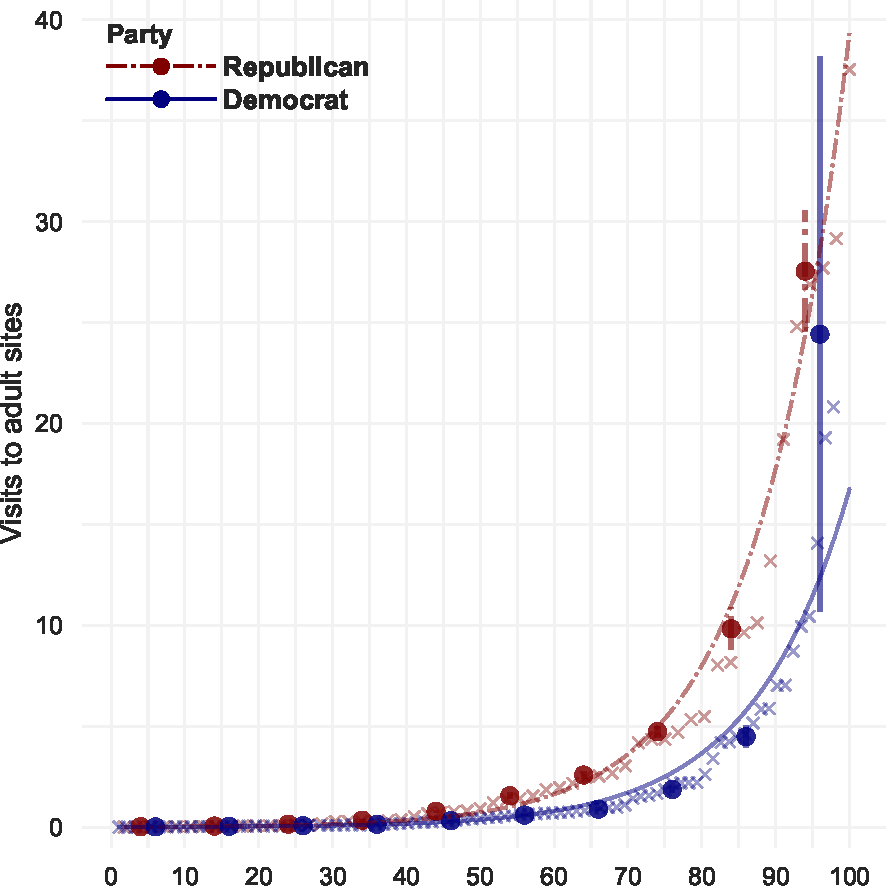
\includegraphics[width=.6\linewidth]{../figs/distribution_duration_on_adultsites_by_party.pdf}
	\caption*{\footnotesize \emph{Notes:} 
		Figure shows splits by party and by percentiles for the total time spent on porn sites for individuals in the sample who consumed pornography in the sample period.
		Round markers and the corresponding vertical lines indicate the mean and 95\% confidence intervals for each bin.
		The \emph{x} symbols indicate actual individuals based on their percentiles.
		See \cref{tab:distribution_duration_party} for the more tabulated values.
	}
	\label{fig:distribution_duration_party}
\end{figure}

%============================================================
% Splits by party for proportion of time spent on adult sites
%============================================================
\begin{figure}[ht]
	\centering
	\caption{Percentage of Time Spent on Pornographic Sites by Party}
	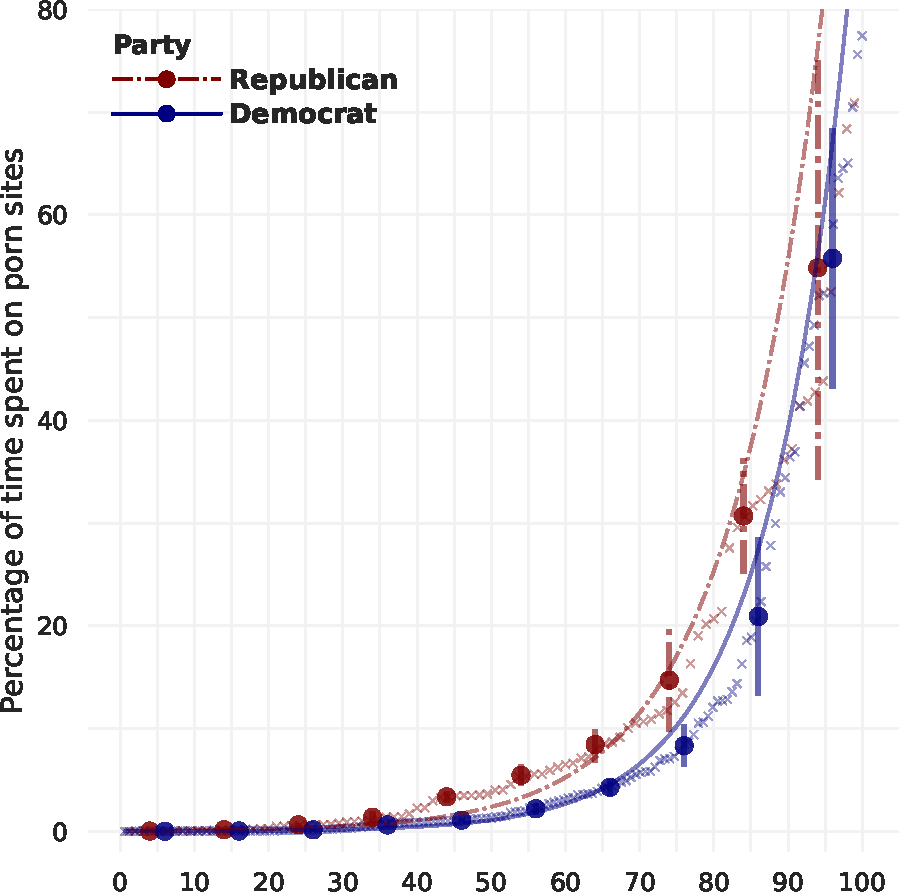
\includegraphics[width=.6\linewidth]{../figs/distribution_proportion_duration_on_adultsites_by_party.pdf}
	\caption*{\footnotesize \emph{Notes:} 
		Figure shows splits by party and by percentiles for the proportion of time spent on porn sites for individuals in the sample who consumed pornography in the sample period.
		Round markers and the corresponding vertical lines indicate the mean and 95\% confidence intervals for each bin.
		The \emph{x} symbols indicate actual individuals based on their percentiles.
		See \cref{tab:distribution_prop_duration_party} for the more tabulated values.
	}
	\label{fig:distribution_prop_duration_party}
\end{figure}

%====================================
% Figure of traffic to top x websites
%====================================
\begin{figure}
	\centering
	\caption{Traffic to Top x Pornographic Sites by Party}
	\includegraphics[width=.6\textwidth]{../figs/concentration_porn_consumption_topX_by_party.pdf}
	\caption*{\footnotesize \emph{Notes:} 
		Figure shows concentration of pornography consumption based on individuals' most frequented pornographic sites.
		Shaded areas are 95\% confidence intervals from bootstrapped standard errors (n = 1,000).
	}
	\label{fig:concentration_porn_consumption_topX_by_party}
\end{figure}


%====================================
% Figure of traffic to top x websites
%====================================
\begin{figure}
	\centering
	\caption{Traffic to Top x Porn Sites by Party}
	\includegraphics[width=.6\textwidth]{../figs/concentration_porn_consumption_topX_by_party.pdf}
	\caption*{\footnotesize \emph{Notes:} 
		Figure shows concentration of porn consumption based on individuals' most frequented porn sites.
		Shaded areas are 95\% confidence intervals from bootstrapped standard errors (n = 1,000).
	}
	\label{fig:concentration_porn_consumption_topX_by_party}
\end{figure}


%==============================================================================
% Fig of quantile regression estimates
% Time Spent on Adult Sites by Party (for individuals who consumed pornography)
%==============================================================================
\begin{figure}[ht]
	\centering
	\caption{Quantile Estimates--Hours Spent on Porn Sites by Party (for individuals who consumed pornography)}
	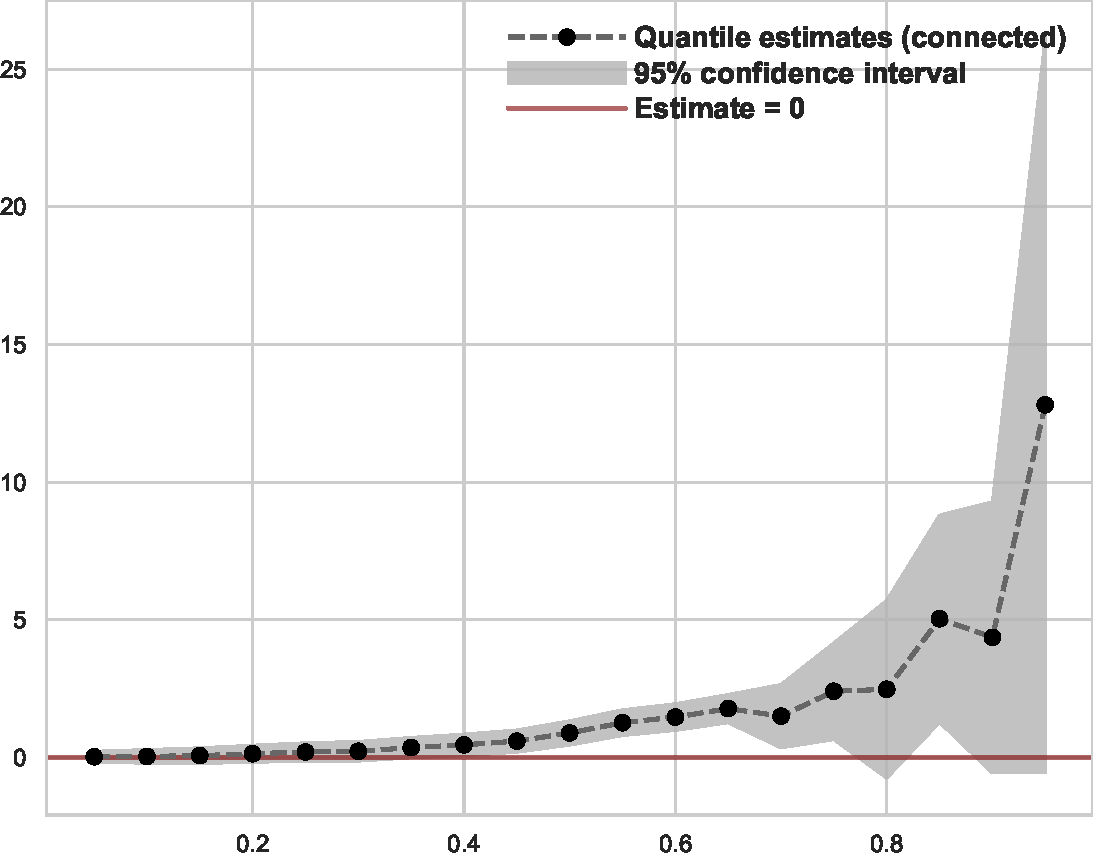
\includegraphics[width=.55\linewidth]{../figs/quantile_reg_nonzero_duration_adult.pdf}
	\caption*{\footnotesize \emph{Notes:} 
		Dependent variable is the number of hours individuals in our sample spent on porn sites.
		Each point indicates the difference between Republicans and Democrats and corresponds to a quantile regression at the quantile indicated by the x-axis.
		Only includes individuals who consumed pornography in the sample period.
		95\% confidence intervals constructed from robust standard errors.
		See \cref{fig:quantile_regression_duration} for the same plot for the full sample.
	}
	\label{fig:quantile_regression_duration_nonzeroes}
\end{figure}

%==============================================================================
% Fig of quantile regression estimates
% Time Spent on Adult Sites by Party (for individuals who consumed pornography and with covariates)
%==============================================================================
\begin{figure}[ht]
	\centering
	\caption{Quantile Estimates--Hours Spent on Porn Sites by Party (for individuals who consumed pornography and with covariates)}
	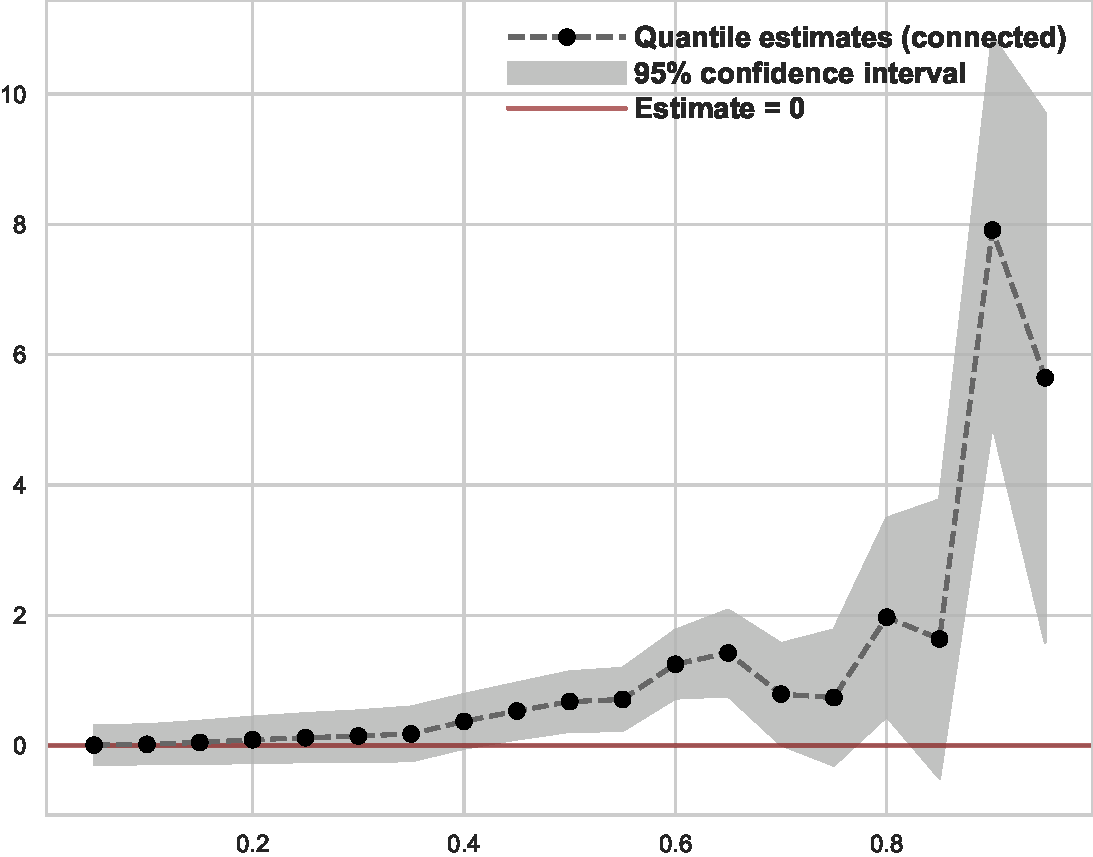
\includegraphics[width=.55\linewidth]{../figs/quantile_reg_nonzero_covariates_duration_adult.pdf}
	\caption*{\footnotesize \emph{Notes:} 
		Dependent variable is the number of hours individuals in our sample spent on porn sites.
		Each point indicates the difference between Republicans and Democrats and corresponds to a quantile regression at the quantile indicated by the x-axis.
		Only includes individuals who consumed pornography in the sample period.
		Covariates included on the right-hand side are: gender (Female/Male), race (White/Black/Hispanic/Asian/Others), education level (no HS/HS graduate/some college/college graduate), age and its quadratic, and region (NE/MW/S/W).
		95\% confidence intervals constructed from robust standard errors.
		See \cref{fig:quantile_regression_duration_covariates} for the same plot for the full sample.
	}
	\label{fig:quantile_regression_duration_nonzeroes_covariates}
\end{figure}



%==============================================================================
% Fig of quantile regression estimates
% Percentage Time Spent on Adult Sites by Party (for individuals who consumed pornography)
%==============================================================================
\begin{figure}[ht]
	\centering
	\caption{Quantile Estimates--Percentage of Time Spent on Porn Sites by Party (for individuals who consumed pornography)}
	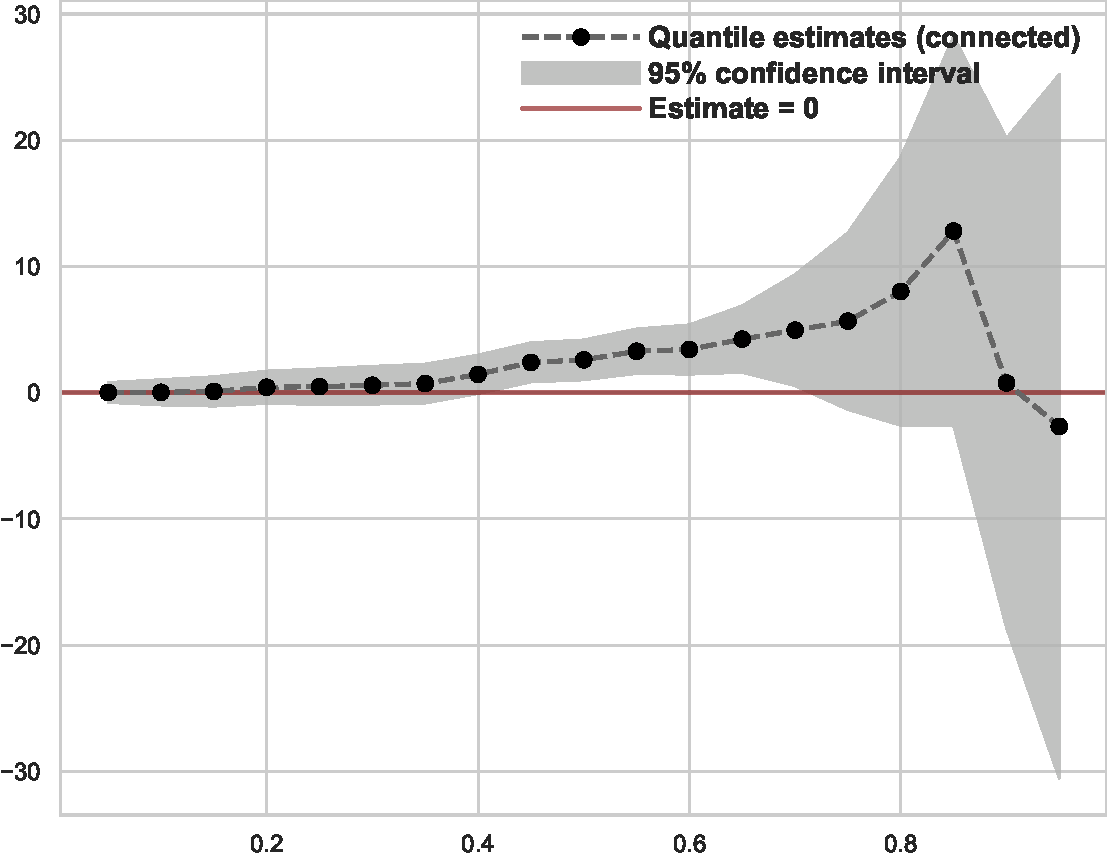
\includegraphics[width=.55\linewidth]{../figs/quantile_reg_nonzero_proportion_duration_adult.pdf}
	\caption*{\footnotesize \emph{Notes:} 
		Dependent variable is the percentage of time individuals in our sample spent on porn sites.
		Each point indicates the difference between Republicans and Democrats and corresponds to a quantile regression at the quantile indicated by the x-axis.
		Only includes individuals who consumed pornography in the sample period.
		95\% confidence intervals constructed from robust standard errors.
		See \cref{fig:quantile_regression_prop_duration} for the same plot for the full sample.
	}
	\label{fig:quantile_regression_prop_duration_nonzeroes}
\end{figure}

%==============================================================================
% Fig of quantile regression estimates
% Time Spent on Adult Sites by Party (for individuals who consumed pornography and with covariates)
%==============================================================================
\begin{figure}[ht]
	\centering
	\caption{Quantile Estimates--Percentage of Time Spent on Porn Sites by Party (for individuals who consumed pornography and with covariates)}
	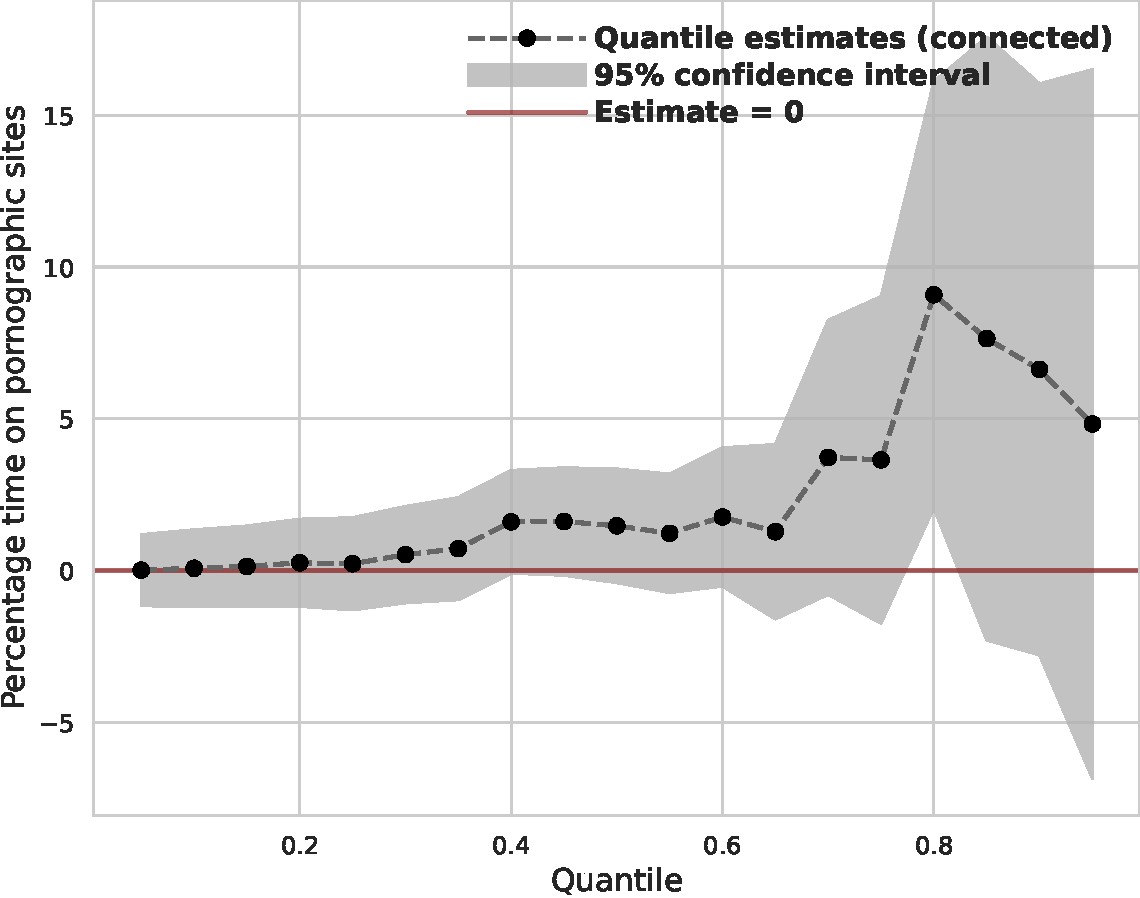
\includegraphics[width=.55\linewidth]{../figs/quantile_reg_nonzero_covariates_proportion_duration_adult.pdf}
	\caption*{\footnotesize \emph{Notes:} 
		Dependent variable is the percentage of time individuals in our sample spent on porn sites.
		Each point indicates the difference between Republicans and Democrats and corresponds to a quantile regression at the quantile indicated by the x-axis.
		Only includes individuals who consumed pornography in the sample period.
		Covariates included on the right-hand side are: gender (Female/Male), race (White/Black/Hispanic/Asian/Others), education level (no HS/HS graduate/some college/college graduate), age and its quadratic, and region (NE/MW/S/W).
		95\% confidence intervals constructed from robust standard errors.
		See \cref{fig:quantile_regression_prop_duration_covariates} for the same plot for the full sample.
	}
	\label{fig:quantile_regression_prop_duration_nonzeroes_covariates}
\end{figure}
\FloatBarrier


%==========================================
% Splits by party for visits to adult sites
%==========================================
\begin{figure}
	\centering
	\caption{Distribution of Traffic to Pornography Online by Party}
	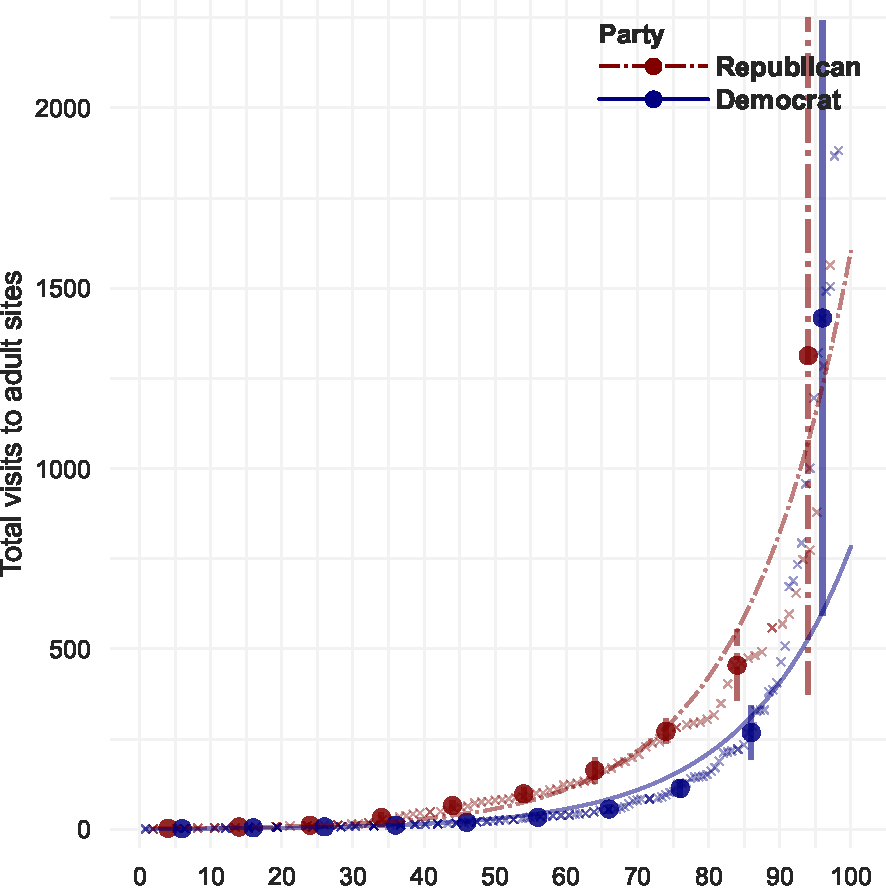
\includegraphics[width=.55\linewidth]{../figs/distribution_visits_to_adultsites_by_party.pdf}
	\caption*{\footnotesize \emph{Notes:} 
		Figure shows splits by party and by percentiles for visits to porn sites for individuals in the sample who consumed pornography in the sample period.
		Round markers and the corresponding vertical lines indicate the mean and 95\% confidence intervals for each bin.
		The \emph{x} symbols indicate actual individuals based on their percentiles.
		See \cref{tab:distribution_visits_party} for the more tabulated values.
	}
	\label{fig:distribution_visits_party}
\end{figure}






%========================================================
% Splits by party for proportion of visits to adult sites
%========================================================
\begin{figure}
	\centering
	\caption{Percentage of Traffic to Pornographic Sites by Party}
	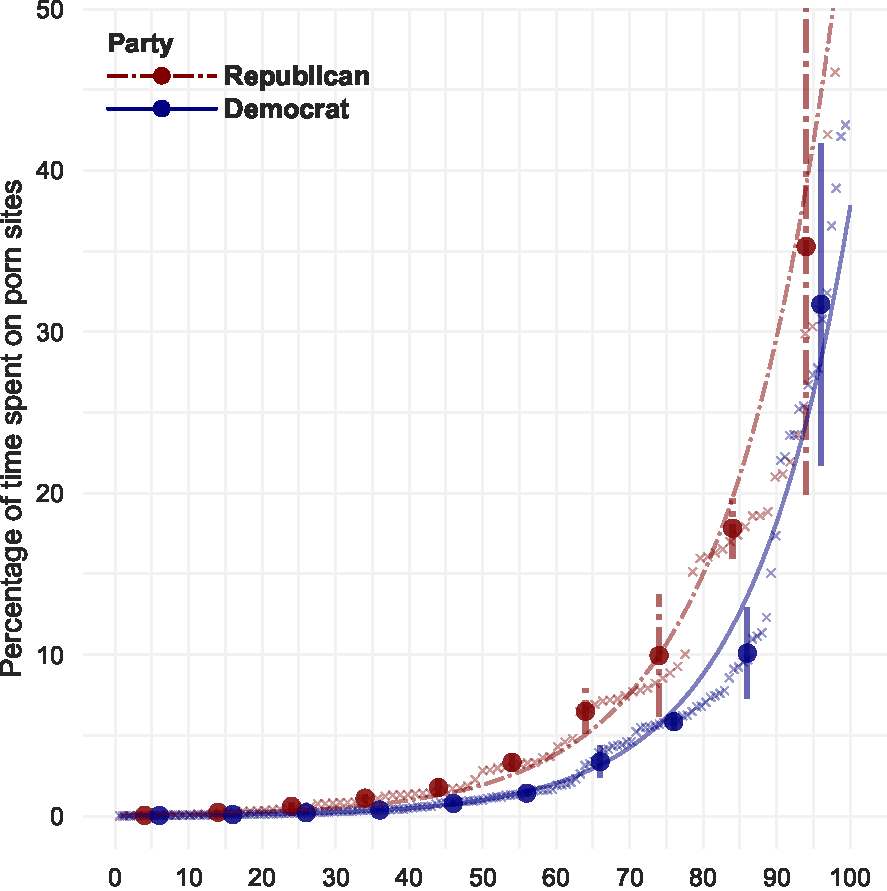
\includegraphics[width=.55\linewidth]{../figs/distribution_proportion_visits_to_adultsites_by_party.pdf}
	\caption*{\footnotesize \emph{Notes:} 
		Figure shows splits by party and by percentiles for visits to porn sites for individuals in the sample who consumed pornography in the sample period.
		Round markers and the corresponding vertical lines indicate the mean and 95\% confidence intervals for each bin.
		The \emph{x} symbols indicate actual individuals based on their percentiles.
		See \cref{tab:distribution_prop_visits_party} for the more tabulated values.
	}
	\label{fig:distribution_prop_visits_party}
\end{figure}





%===============================================
% Tabulated percentiles of visits to adult sites
%===============================================
\begin{table} \centering \small \setlength\tabcolsep{10 pt}
	\caption{Distribution of Traffic to Pornography Online}
	\label{tab:distribution_visits}
	\begin{adjustbox}{max width=\textwidth}
		\begin{tabular}{cr}
			\toprule
			\multicolumn{1}{c}{\textbf{Percentile}}&\multicolumn{1}{c}{\textbf{Visits}}\\
			\midrule
			0.00 &    1 \\
0.10 &    4 \\
0.20 &    7 \\
0.30 &   12 \\
0.40 &   25 \\
0.50 &   46 \\
0.60 &   77 \\
0.70 &  134 \\
0.80 &  262 \\
0.90 &  524 \\
0.95 & 1158 \\
0.96 & 1459 \\
0.97 & 1841 \\
0.98 & 2315 \\
0.99 & 2830 \\
1.00 & 4264 \\
			\bottomrule
		\end{tabular}
	\end{adjustbox}
	\caption*{\footnotesize \emph{Notes:} 
		Table shows key percentiles (each of the ten deciles plus quantiles at the right tail) and their corresponding values for traffic to porn sites by individuals who consumed pornography in the sample period. 
		See \cref{fig:distribution_visits} for the plot.
	}
\end{table}




%=============================================================
% Tabulated percentiles of proportion of visits to adult sites
%=============================================================
\begin{table} \centering \small \setlength\tabcolsep{10 pt}
	\caption{Percentage of Traffic to Pornographic Sites}
	\label{tab:distribution_prop_visits}
	\begin{adjustbox}{max width=\textwidth}
		\begin{tabular}{cr}
			\toprule
			\multicolumn{1}{c}{\textbf{Percentile}}&\multicolumn{1}{c}{\textbf{\% visits}}\\
			\midrule
			0.00 &  0.0 \\
0.10 &  0.1 \\
0.20 &  0.2 \\
0.30 &  0.5 \\
0.40 &  1.0 \\
0.50 &  1.6 \\
0.60 &  3.7 \\
0.70 &  6.3 \\
0.80 &  9.7 \\
0.90 & 22.0 \\
0.95 & 31.4 \\
			\bottomrule
		\end{tabular}
	\end{adjustbox}
	\caption*{\footnotesize \emph{Notes:} 
		Table shows key percentiles (each of the ten deciles plus quantiles at the right tail) and their corresponding values for traffic to porn sites by individuals who consumed pornography in the sample period. 
		See \cref{fig:distribution_prop_visits} for the plot.
	}
\end{table}




%======================================================================
% Tabulated splits by party and by percentiles for visits to adultsites
%======================================================================
\begin{table} \centering \small \setlength\tabcolsep{10 pt}
	\caption{Distribution of Traffic to Pornography Online by Party}
	\label{tab:distribution_visits_party}
	\begin{adjustbox}{max width=\textwidth}
		\begin{tabular}{crr}
			\toprule
			\multicolumn{1}{l}{\textbf{}}&\multicolumn{2}{c}{\textbf{Visits}}\\
			\cmidrule(l){2-3}
			\multicolumn{1}{l}{\textbf{Percentile}}&\multicolumn{1}{c}{\textbf{Republicans}}&\multicolumn{1}{c}{\textbf{Democrats}}\\			
			\midrule
			0.00 &     1 &     1 \\
0.10 &     4 &     2 \\
0.20 &     9 &     5 \\
0.30 &    15 &     9 \\
0.40 &    48 &    14 \\
0.50 &    82 &    25 \\
0.60 &   125 &    39 \\
0.70 &   210 &    82 \\
0.80 &   310 &   157 \\
0.90 &   566 &   452 \\
0.95 &   863 & 1,246 \\
0.96 & 1,235 & 1,425 \\
0.97 & 1,539 & 1,503 \\
0.98 & 2,348 & 1,875 \\
0.99 & 2,414 & 2,465 \\
1.00 & 2,560 & 3,980 \\
			\bottomrule
		\end{tabular}
	\end{adjustbox}
	\caption*{\footnotesize \emph{Notes:} 
		Table shows splits by party and by key percentiles (each of the ten deciles plus quantiles at the right tail) for traffic to porn sites by individuals who consumed pornography in the sample period. See \cref{fig:distribution_visits_party} for the plot.
	}
\end{table}




%===============================================================================
% Tabulated splits by party and by percentiles for proportion of time spent on adultsites
%===============================================================================
\begin{table} \centering \small \setlength\tabcolsep{10 pt}
	\caption{Percentage of Traffic to Pornographic Sites by Party}
	\label{tab:distribution_prop_visits_party}
	\begin{adjustbox}{max width=\textwidth}
		\begin{tabular}{@{\hspace{0\tabcolsep}}ccc@{\hspace{0\tabcolsep}}}
			\toprule
			\multicolumn{1}{l}{\textbf{}}&\multicolumn{2}{c}{\textbf{\% visits}}\\
			\cmidrule(l){2-3}
			\multicolumn{1}{l}{\textbf{Percentile}}&\multicolumn{1}{c}{\textbf{Republicans}}&\multicolumn{1}{c}{\textbf{Democrats}}\\	
			\midrule
			0.00 &  0.0 &  0.0 \\
0.10 &  0.1 &  0.1 \\
0.20 &  0.4 &  0.1 \\
0.30 &  0.8 &  0.3 \\
0.40 &  1.4 &  0.5 \\
0.50 &  2.8 &  1.0 \\
0.60 &  4.3 &  1.9 \\
0.70 &  7.7 &  4.6 \\
0.80 & 16.0 &  7.0 \\
0.90 & 21.1 & 18.8 \\
0.95 & 30.5 & 27.4 
% 0.96 & 32.7 & 29.9 \\
% 0.97 & 42.6 & 33.6 \\
% 0.98 & 46.5 & 38.6 \\
% 0.99 & 52.8 & 42.4 \\
% 1.00 & 53.5 & 59.9 \\
			\bottomrule
		\end{tabular}
	\end{adjustbox}
	\caption*{\footnotesize \emph{Notes:} 
		Table shows splits by party and by key percentiles (each of the ten deciles plus quantiles at the right tail) for traffic to porn sites by individuals who consumed pornography in the sample period. See \cref{fig:distribution_prop_visits_party} for the plot.
	}
\end{table}

%==============================================================================
% Fig of quantile regression estimates
% Percentage Traffic to Adult Sites by Party (for individuals who consumed pornography)
%==============================================================================
\begin{figure}
	\centering
	\caption{Quantile Estimates--Percentage of Traffic to Porn Sites by Party (for individuals who consumed pornography)}
	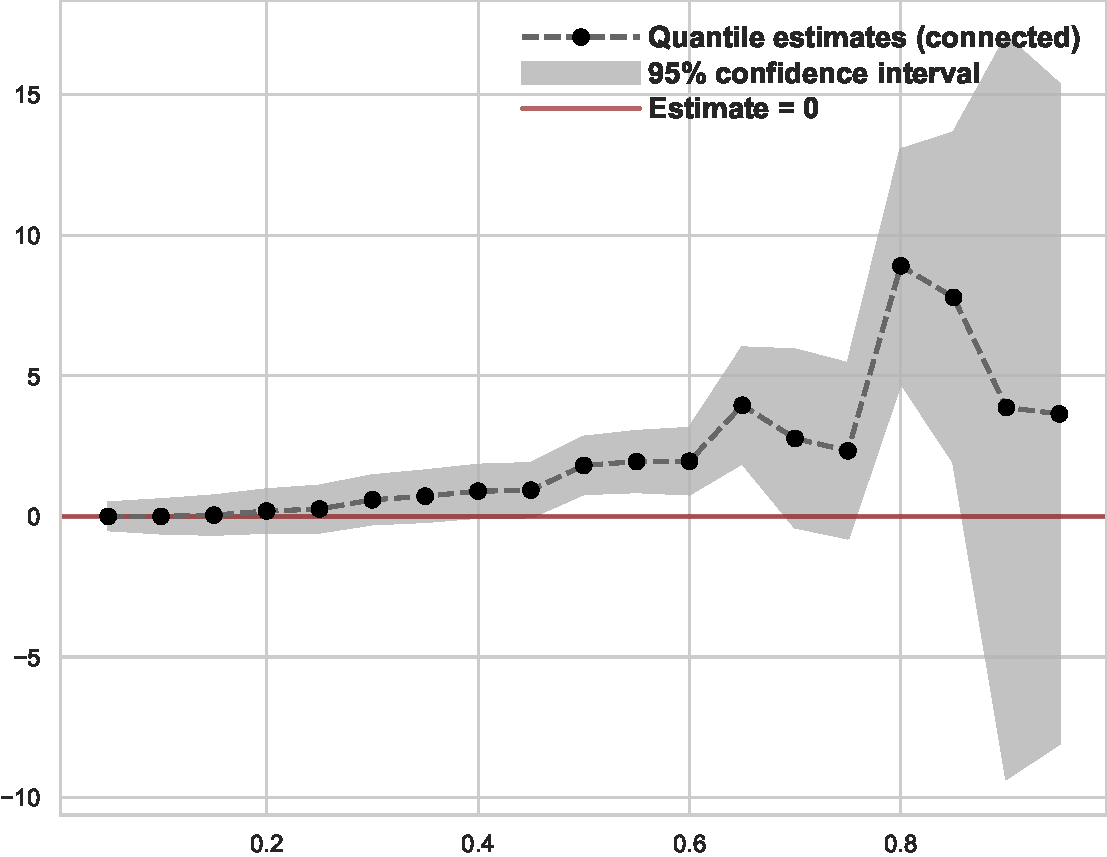
\includegraphics[width=.55\linewidth]{../figs/quantile_reg_nonzero_proportion_visits_adult.pdf}
	\caption*{\footnotesize \emph{Notes:} 
		Dependent variable is the percentage of traffic to porn sites by individuals in our sample.
		Each point indicates the difference between Republicans and Democrats and corresponds to a quantile regression at the quantile indicated by the x-axis.
		Only includes individuals who consumed pornography in the sample period.
		95\% confidence intervals constructed from robust standard errors.
		See \cref{fig:quantile_regression_prop_visits} for the same plot for the full sample.
	}
	\label{fig:quantile_regression_prop_visits_nonzeroes}
\end{figure}



%==============================================================================
% Fig of quantile regression estimates
% Percentage Traffic to Adult Sites by Party (for individuals who consumed pornography and with covariates)
%==============================================================================
\begin{figure}
	\centering
	\caption{Quantile Estimates--Percentage of Traffic to Porn Sites by Party (for individuals who consumed pornography and with covariates)}
	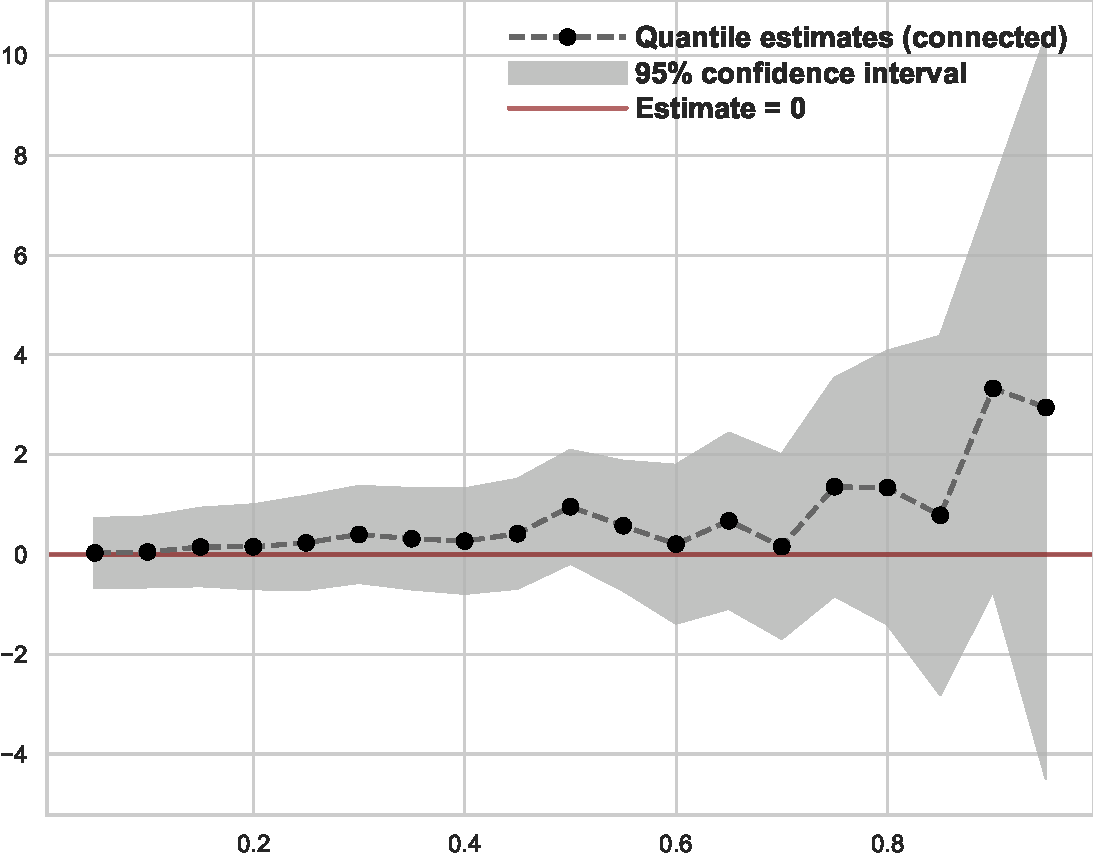
\includegraphics[width=.55\linewidth]{../figs/quantile_reg_nonzero_covariates_proportion_visits_adult.pdf}
	\caption*{\footnotesize \emph{Notes:} 
		Dependent variable is the percentage of traffic to porn sites by individuals in our sample.
		Each point indicates the difference between Republicans and Democrats and corresponds to a quantile regression at the quantile indicated by the x-axis.
		Only includes individuals who consumed pornography in the sample period.
		Covariates included on the right-hand side are: gender (Female/Male), race (White/Black/Hispanic/Asian/Others), education level (no HS/HS graduate/some college/college graduate), age and its quadratic, and region (NE/MW/S/W).
		95\% confidence intervals constructed from robust standard errors.
		See \cref{fig:quantile_regression_prop_visits_covariates} for the same plot for the full sample.
	}
	\label{fig:quantile_regression_prop_visits_nonzeroes_covariates}
\end{figure}

%==============================================================================
% Fig of quantile regression estimates
% Traffic to Adult Sites by Party (for individuals who consumed pornography and with covariates)
%==============================================================================
\begin{figure}
	\centering
	\caption{Quantile Estimates--Traffic to Porn Sites by Party (for individuals who consumed pornography and with covariates)}
	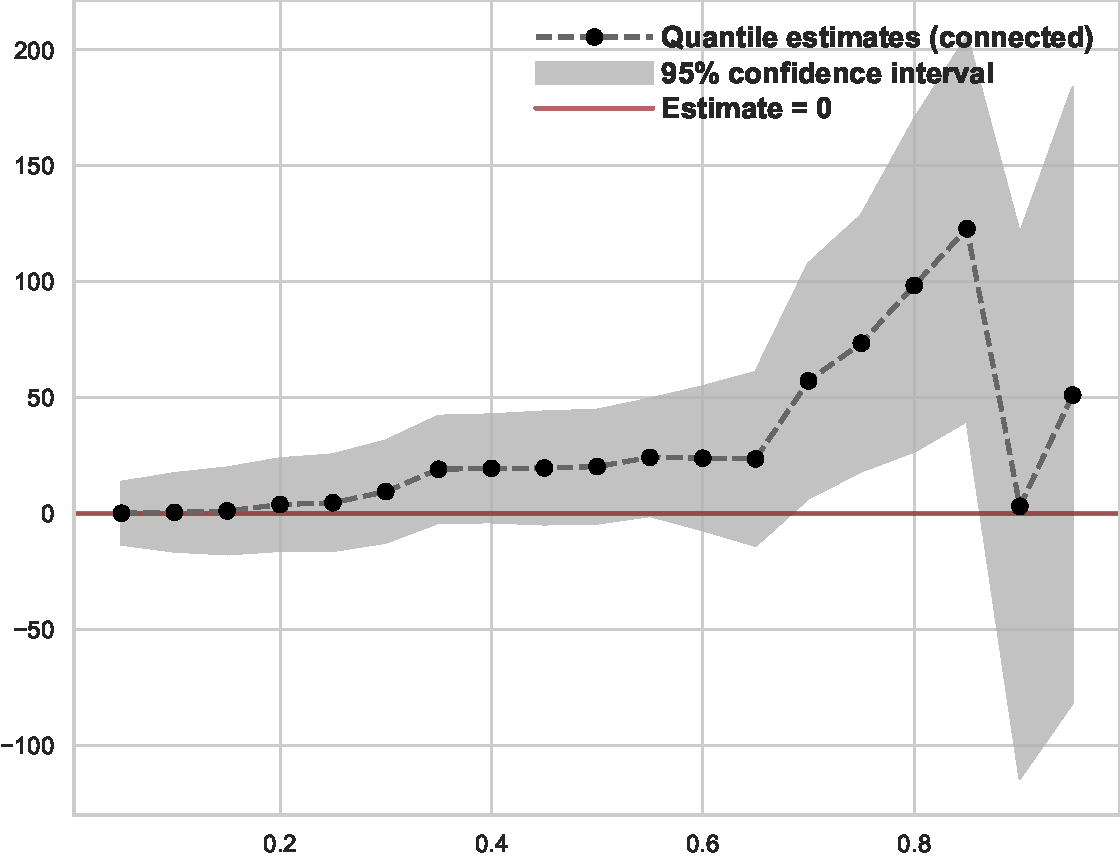
\includegraphics[width=.55\linewidth]{../figs/quantile_reg_nonzero_covariates_visits_adult.pdf}
	\caption*{\footnotesize \emph{Notes:} 
		Dependent variable is the number of visits to porn sites by individuals in our sample.
		Each point indicates the difference between Republicans and Democrats and corresponds to a quantile regression at the quantile indicated by the x-axis.
		Only includes individuals who consumed pornography in the sample period.
		Covariates included on the right-hand side are: gender (Female/Male), race (White/Black/Hispanic/Asian/Others), education level (no HS/HS graduate/some college/college graduate), age and its quadratic, and region (NE/MW/S/W).
		95\% confidence intervals constructed from robust standard errors.
		See \cref{fig:quantile_regression_visits_covariates} for the same plot for the full sample.
	}
	\label{fig:quantile_regression_visits_nonzeroes_covariates}
\end{figure}

%===========================================================================
% Fig of quantile regression estimates
% Traffic to Adult Sites by Party (for individuals who consumed pornography)
%===========================================================================
\begin{figure}
	\centering
	\caption{Quantile Estimates--Traffic to Porn Sites by Party (for individuals who consumed pornography)}
	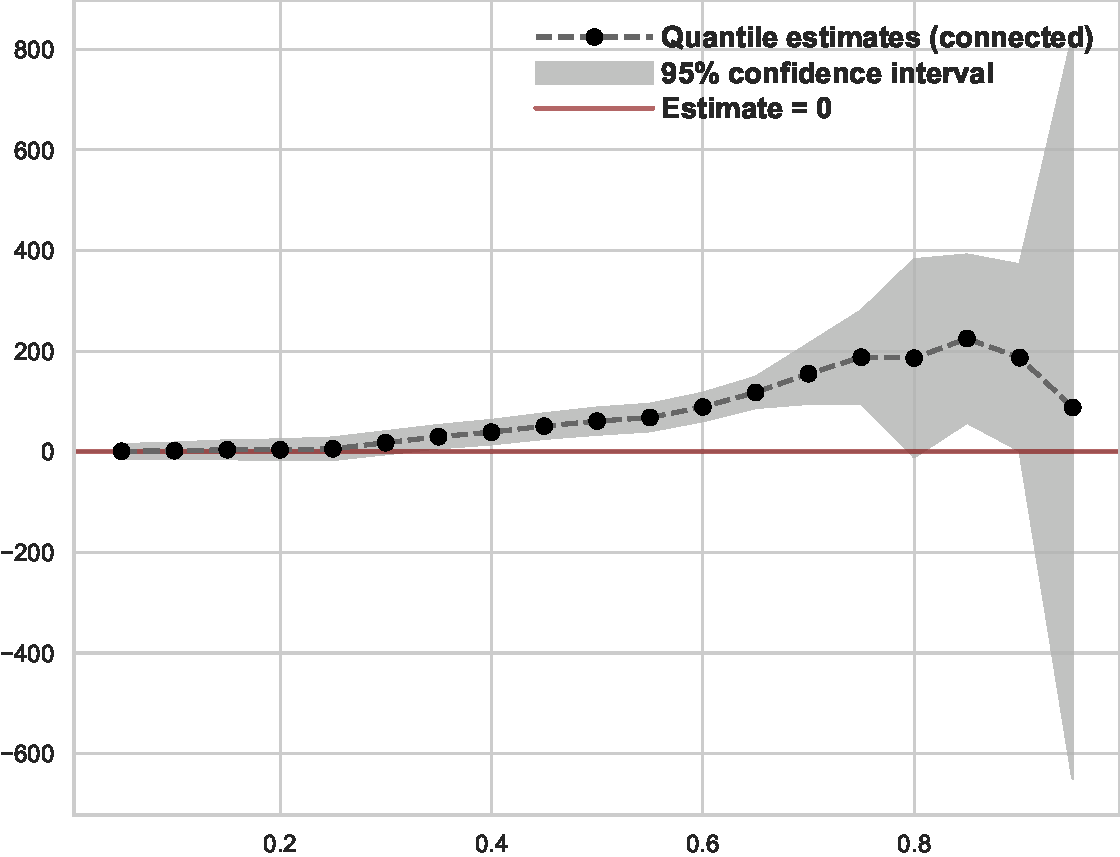
\includegraphics[width=.55\linewidth]{../figs/quantile_reg_nonzero_visits_adult.pdf}
	\caption*{\footnotesize \emph{Notes:} 
		Dependent variable is the number of visits to porn sites by individuals in our sample.
		Each point indicates the difference between Republicans and Democrats and corresponds to a quantile regression at the quantile indicated by the x-axis.
		Only includes individuals who consumed pornography in the sample period.
		95\% confidence intervals constructed from robust standard errors.
		See \cref{fig:quantile_regression_visits} for the same plot for the full sample.
	}
	\label{fig:quantile_regression_visits_nonzeroes}
\end{figure}
